\documentclass[12pt]{article}
\usepackage{graphicx}
\begin{document}
\noindent \textbf{TO}: Bruce Bolden\par 
\noindent
\textbf{FROM}: Group 2, CS-383 Class\par 
\noindent
\textbf{DATE}: September 2, 2016\par 
\noindent
\section*{Abstract}
The following is the specification and time line of our Tower of Lights project.
\section*{The First Iteration}
The program should have/be able to...\begin{itemize}
\item{open, save, and create new .tan files}
\item{an exit feature}
\item{gridlayout used to view a frame}
\end{itemize}
\section*{Details}
The first iteration will be able to open animation files and determine if a given file is actually a .tan file. The iteration will not be able to show the animation file. Instead we will be only adding the grid interface in which we will later add the functionality to view the frames in the project. The save feature will be added for .tan files. We will also include an exit button in this first iteration of the program. 
\section*{Rough  Time line}
1st iteration (due by Nov. 9 2016)\par 
\noindent
2nd iteration (due by Nov. 16 2016)\par 
\noindent
3rd iteration (due by Nov. 23 2016)\par 
\noindent
4th iteration (due by Nov. 30 2016)\par 
\noindent
final iteration...due by Dec. 7 2016\par 
\noindent
\pagebreak
\noindent
%%
%%
\section*{Appendix}
\subsection*{Further Iterations' Details}
Iteration 2\par
\noindent
\begin{itemize}
\item{select cells}
\item{select colors}
\end{itemize}
Iteration 3\par
\noindent
\begin{itemize}
\item{frame manipulation}
\item{add frame time interval}
\item{frame previewer}
\end{itemize}
Iteration 4\par
\noindent
\begin{itemize}
\item{select audio file}
\item{animation preview}
\end{itemize}
Iteration final\par
\noindent
\begin{itemize}
\item{effects}
\item{patterns}
\end{itemize}
\subsection*{Iteration 1 Interface}
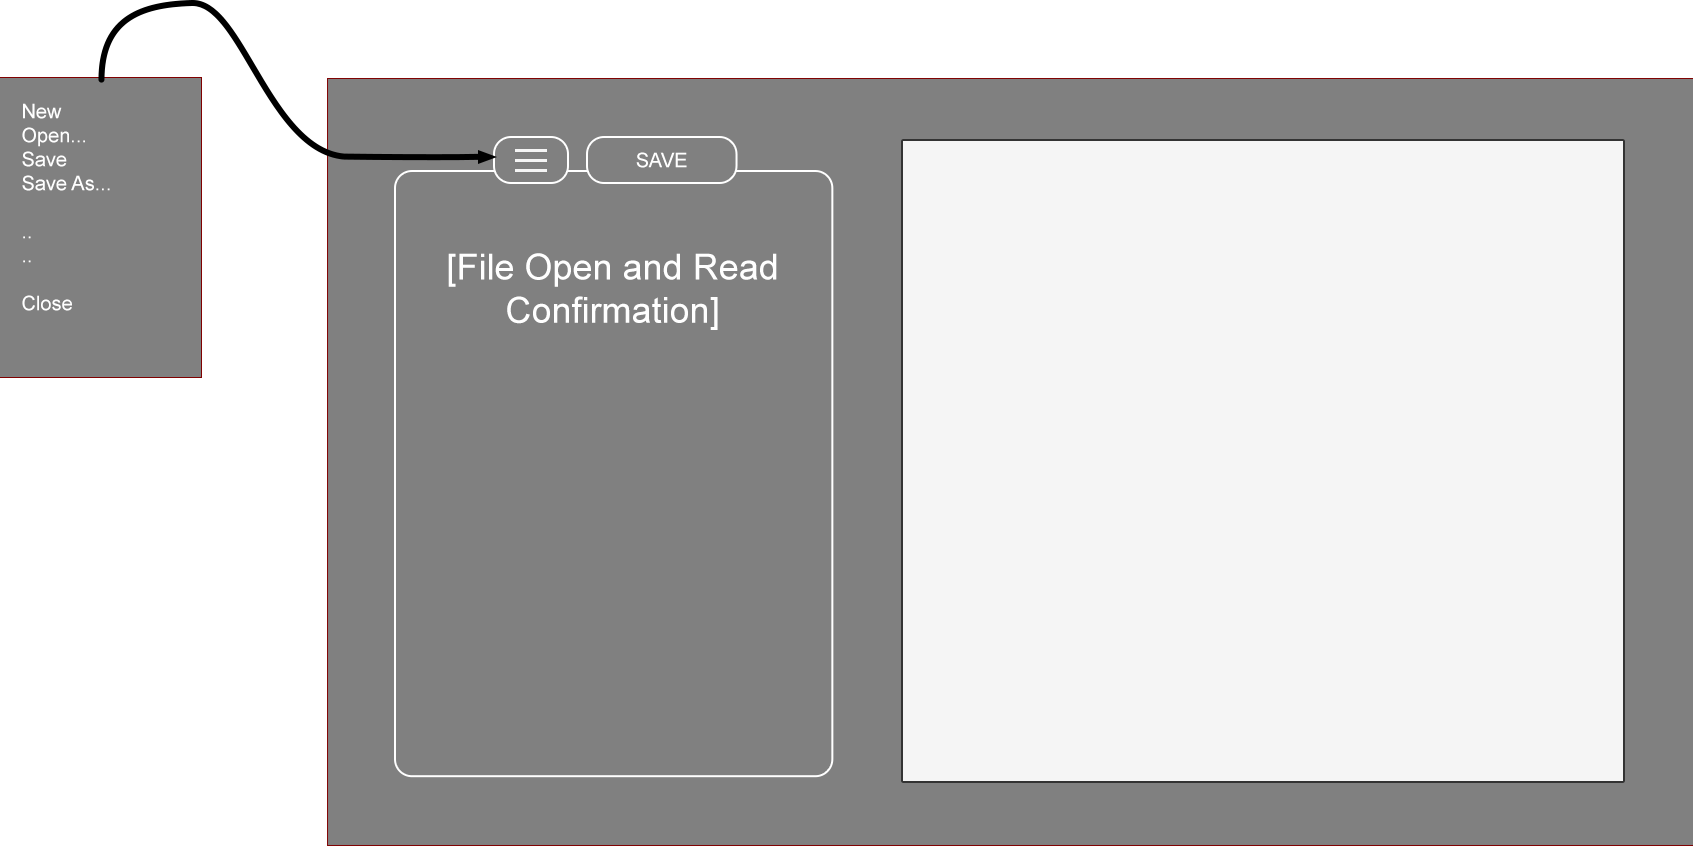
\includegraphics[scale=.25]{CS336-Project01-UI-Week1_Target.png}
\subsection*{Final Interface}
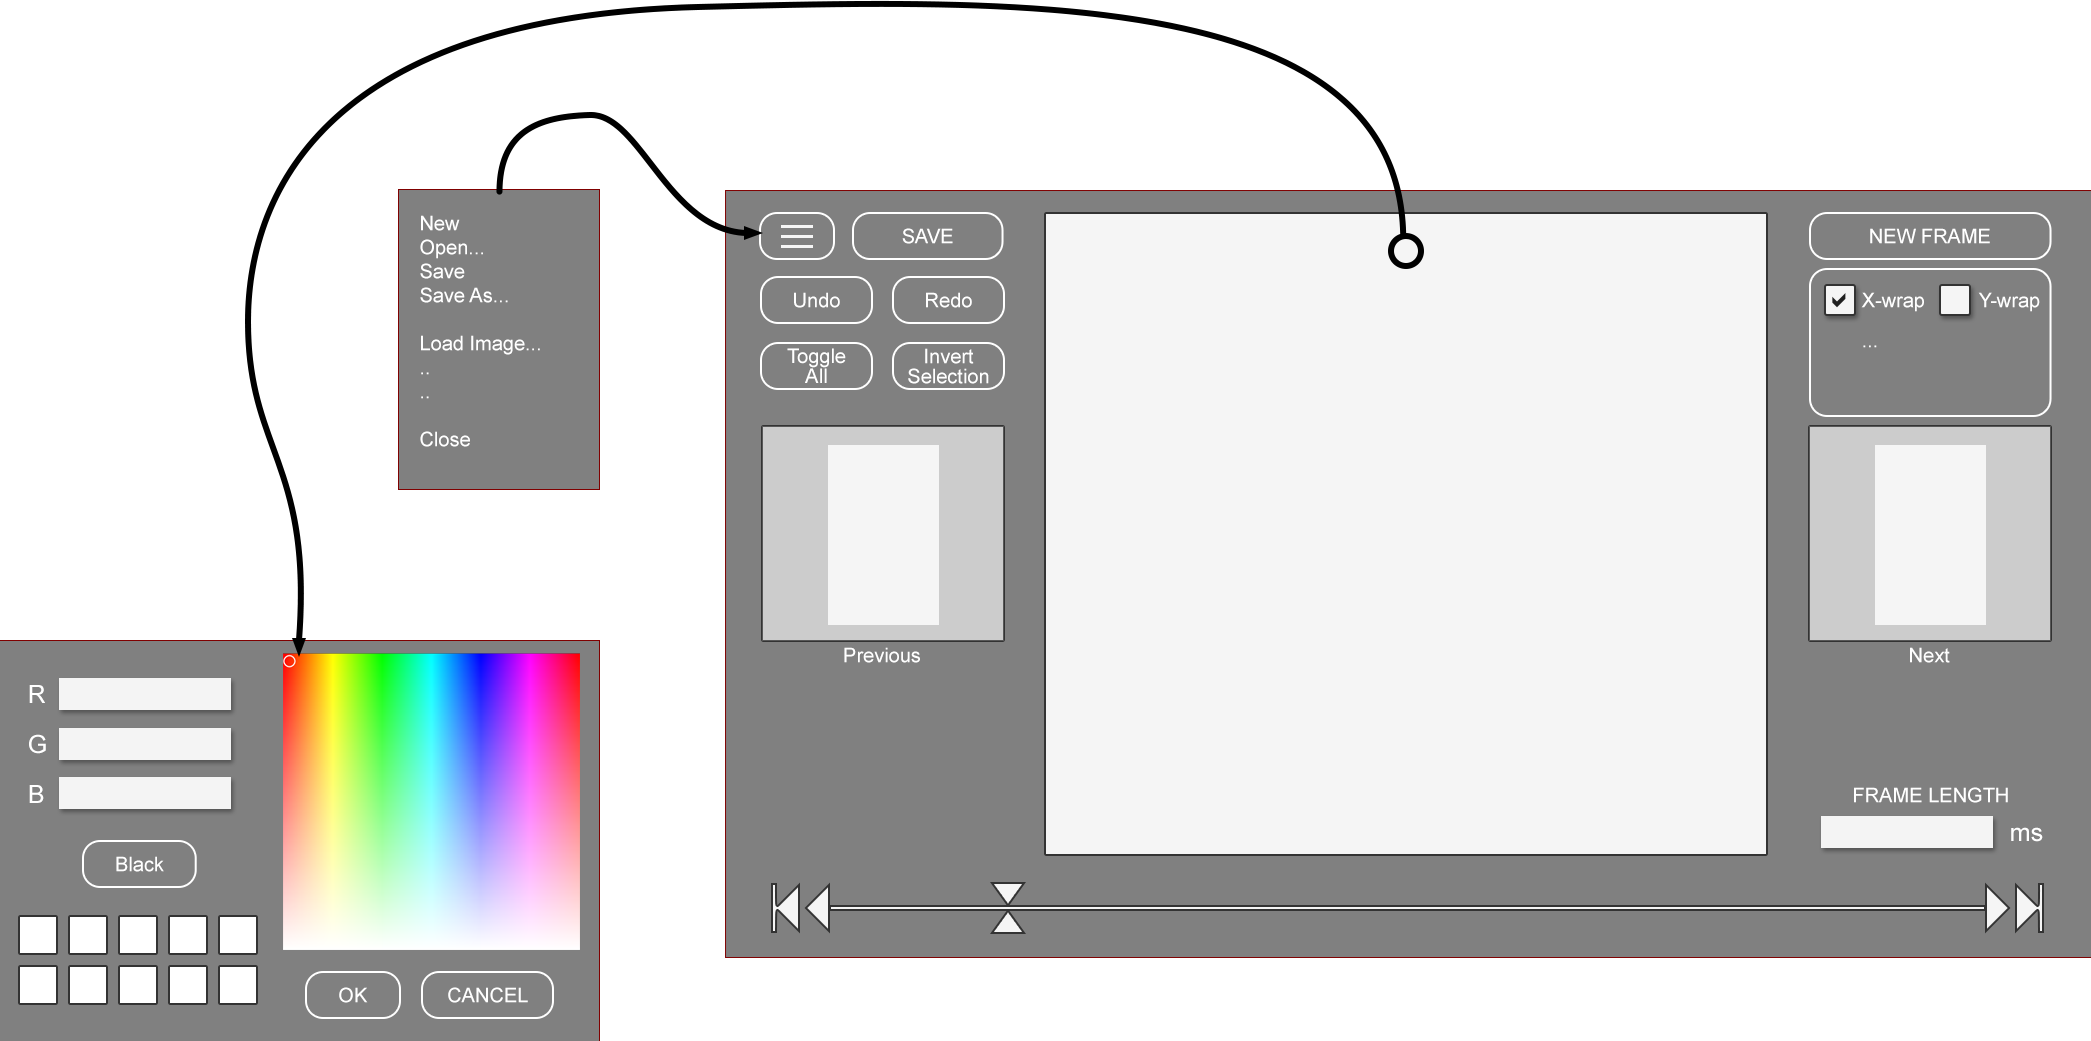
\includegraphics[scale=.19]{CS336-Project01-UI.png}
\subsection*{Iteration 1 Use Cases}
Open file (.tan) - pop-up box
New file - pop-up box
Save file - pop-up box
Exit program - button
Pop-up Box (Used for a use case which could require extra options)\par
\noindent
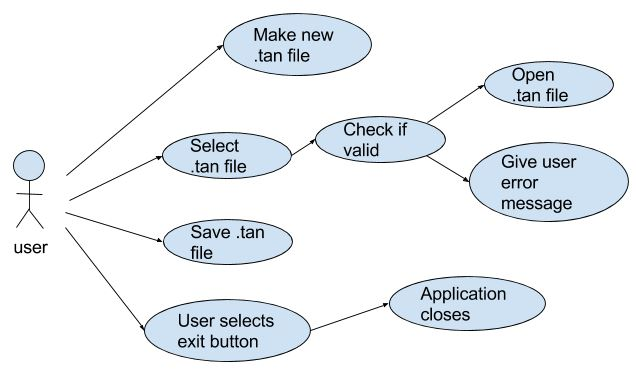
\includegraphics[scale=.82]{UseCases.JPG}
\end{document}
